%% Section 6, Bimanual dexterous manipulation. Converted from paper/sections/06_bimanual.md.
\section{Bimanual dexterous manipulation}
\label{sec:bimanual}

% --- reproduced plates ------------------------------------------------------
% tex/figs/plates.tex defines one command per selected photograph. Load it here
% if nothing has loaded it already, so this section carries its own plates
% whether or not the preamble inputs the file. The \providecommand before each
% call makes a missing plate an empty command rather than an error. Every plate
% carries \pending: read tex/PERMISSIONS.md before this goes anywhere.
% ---------------------------------------------------------------------------
\makeatletter
\@ifundefined{plateGraspPenetration}{\IfFileExists{figs/plates.tex}{% The one reproduced plate.
% Rebuilt from its source PDF by tools/relayout_plates.py; see tex/figs/SELECTED.md for the crop
% box and tex/PERMISSIONS.md for the licence it is used under.
%
% A plate is kept only where a photograph or a render carries something a drawing cannot, and
% only where the paper has the right to print it without asking anyone. Everything else that was
% reproduced has been redrawn in the paper's own style (figs/fig_transmission, fig_collision,
% fig_tactiledepth, fig_contactlabel, fig_retarget) or dropped, because the prose already made the
% point or because no honest drawing could be made from what the corpus records. That took
% eighteen plates to one, eleven visual styles to four, and eleven open permissions to none.
%
% The survivor is single column and single panel. It is not a `figure*`: a borrowed plate has not
% earned the page width.
%
% One command for it. A section author places it by writing
%   \plateGraspPenetration
% at the point in the section where the float should be anchored, once: a plate called twice
% prints twice, on two pages, under two numbers.
%
% The plate credits its source inside its own caption with \src or \cite, and carries \licensed as
% well, because its source is CC BY 4.0 and the licence asks for an attribution line.

% ========================================================== Sec. VI, two hands

\newcommand{\plateGraspPenetration}{%
  \begin{figure}[t]
    \centering
    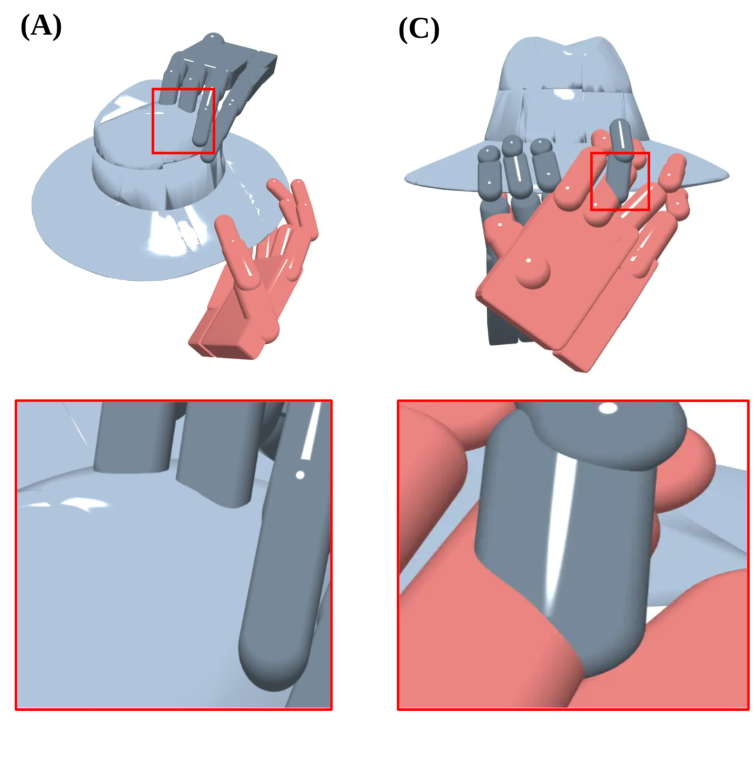
\includegraphics[width=0.86\columnwidth]{figs/selected/bimanual_grasp_penetration.png}
    \caption{Two failures of synthesised two-hand grasps, each enlarged at the
      contact: (A) a finger inside the object, (C) a finger inside the other hand.
      Both look plausible whole~\cite{bimangrasp_2024}.}
    \label{fig:bimanual-penetration}
    \licensed[panels (A) and (C) of Fig.~9]{Fig.~9 of Shao and Xiao, arXiv:2411.15903}{CC BY 4.0}{https://creativecommons.org/licenses/by/4.0/}
  \end{figure}}
}{}}{}
\makeatother

A warning first. Fifty-three corpus method rows carry the two-hand flag, and that flag says only
that the robot has two end effectors. Thirteen of the 53 put no dexterous hand on the robot at
all. ALOHA, RDT-1B, EgoMimic and H-RDT \cite{aloha_act_2023,rdt1b_2024,egomimic_2024,h_rdt_2025}
and UMI \cite{umi_2024} are parallel-jaw throughout; $\pi_0$, $\pi_{0.5}$ and $\pi^{*}_{0.6}$
\cite{pi0_2024,pi05_2025,pistar06_2025} and Diffusion Policy \cite{diffusion_policy_2023} name no
hand and run grippers on every embodiment; Gemini Robotics \cite{gemini_robotics_2025} and Gemini
Robotics 1.5 \cite{gemini_robotics_15_2025} report every bimanual number on grippers and show
five-fingered hands only qualitatively; and Helix \cite{helix_2025} and GR00T N1.6
\cite{groot_n16_2025} name no end effector anywhere on the page. Three more run a gripper on one
embodiment and a hand on another: ACE and 3D Diffusion Policy \cite{ace_teleop_2024,dp3_2024} and
Open-TeleVision \cite{open_television_2024}, whose Unitree H1 carries 6-DoF Inspire hands and
whose Fourier GR-1 carries a 1-DoF jaw.

\textbf{The denominator for this section is 28}: the method rows whose notes place a learned
closed-loop controller on two multi-fingered hands. It is the 53 less those 16; less two static
grasp-synthesis methods, BimanGrasp \cite{bimangrasp_2024} and BiDexGrasp \cite{bidexgrasp_2026};
less three systems with no learned policy, Castro et al. and DexTeleop-0
\cite{castro_sap_contact_2021,dexteleop0_2026} and Pang et al. \cite{pang_global_planning_2022};
and less four rows where no learned policy holds both hands: OmniH2O \cite{omnih2o_2024}, whose
fingers are mapped open-loop from the Vision Pro and sit outside its 19-DoF policy; OKAMI
\cite{okami_2024}, whose headline pipeline is open-loop retargeting with a learned policy only in
a side experiment; DexDeform \cite{dexdeform_2023}, a skill model refined by trajectory
optimisation rather than a closed-loop controller; and Omnigrasp \cite{omnigrasp_2024}, a
simulated human body with no bimanual task. Frau-Alfaro et al. \cite{dexterous_handover_2025}
never enter, because their row records one hand. Benchmarks and datasets are outside the 28 by
class, Bi-DexHands and Bench2Dex \cite{bidexhands_2022,bench2dex_2026} and RoboPianist
\cite{robopianist_2023} being benchmarks and RP1M \cite{rp1m_2024} and HumanoidGen
\cite{humanoidgen_2025} datasets; they are quoted here as evidence and never counted. Every paper
below runs two multi-fingered hands unless said otherwise.

\subsection{Why two hands is not twice one hand}
\label{subsec:two_not_twice}

When both hands hold the same object, the object closes a kinematic loop between them. Neither
hand can move without changing what the other must do. BiDexGrasp \cite{bidexgrasp_2026} reports
that the coupled objective ``often yields imbalanced solutions, where one hand dominates stability
while the other contributes marginally.'' ArtiGrasp \cite{artigrasp_2023} reports simulation speed
scaling ``roughly quadratically with the number of contacts,'' and trains each hand alone before
pairing them.

Role asymmetry is an assumption almost everyone makes silently. BiDexHD \cite{bidexhd_2024} states
it outright: ``we assume the robot to be right-handed by default, i.e., the left hand handles the
target object and the right hand handles the tool,'' and Lin et al. \cite{twisting_lids_2024} bake
the same split into their reward, putting reference contact keypoints on the bottle base for the
left fingertips and on the lid for the right. The bias is in the data first: TACO \cite{taco_2024}
recruited 14 right-handed subjects and measures the right hand moving consistently faster.

The arms collide, and the corpus handles this by construction rather than by control. RoboPianist
\cite{robopianist_2023} ships a forearm-forearm collision term that its own reward table never
lists. Two papers name arm collision as unsolved. DexMimicGen \cite{dexmimicgen_2024} ``does not
explicitly handle collisions,'' and DexMan \cite{dexman_2025} says its control parameterisation
``overlooks full arm posture,'' which it needs to avoid them.

The action space doubles and the observation grows faster. Bi-DexHands \cite{bidexhands_2022} uses
a 52-dimensional action for 18 of its 20 tasks against observations of 398 to 446 dimensions.
GR-Dexter \cite{gr_dexter_2025} emits an 88-dimensional chunk of arm joints, end-effector poses,
hand joints and fingertips. What the larger vector does not carry is any statement of who does
what. The usual answer is one scalar reward summed over both sides, and the cost is a compounding
failure rate. ManipTrans \cite{maniptrans_2025} scores success only if both hands succeed, and its
OakInk-V2 success rate falls from 58.1 percent on single-hand sequences to 39.5 percent on
bimanual ones.

\subsection{Coordination architectures}
\label{subsec:coordination}

\begin{figure*}[!t]
\centering
\IfFileExists{figs/fig_bimanual.tex}{% hand-drawn to match the style of tools/make_tikz_figures.py output
% Four coordination architectures for two dexterous hands. Greyscale plus the
% one accent; thin rules; square corners. Drawn at two-column width.
\begin{tikzpicture}[
  font=\footnotesize,
  panel/.style={draw=rule,line width=0.4pt,inner sep=0pt},
  panelacc/.style={draw=accent,line width=0.8pt,inner sep=0pt},
  box/.style={draw=black!45,fill=wash,line width=0.3pt,inner sep=0pt,align=center},
  hand/.style={draw=black!55,fill=wash,line width=0.3pt,circle,inner sep=0pt,minimum size=5.0mm,
               font=\tiny},
  handbig/.style={hand,draw=accent,line width=0.5pt,minimum size=6.6mm},
  lnk/.style={draw=black!50,line width=0.35pt,-latex},
  soft/.style={draw=black!45,line width=0.35pt,dash pattern=on 1.4pt off 1.4pt},
  hd/.style={font=\footnotesize\bfseries,align=center,anchor=north},
  cnt/.style={font=\scriptsize\bfseries\color{accent},anchor=north},
  dsc/.style={font=\tiny\color{black!60},align=center,anchor=north},
  ky/.style={font=\tiny\ttfamily\color{black!75},align=center,anchor=north},
]

% ---------------------------------------------------------------- panel 1 ----
\begin{scope}[shift={(0,0)}]
  \node[panelacc,minimum width=42mm,minimum height=40mm] at (2.1,2.00) {};
  \node[hd] at (2.1,3.86) {one policy, both hands};
  \node[cnt] at (2.1,3.56) {21 of 28};
  \node[dsc] at (2.1,3.32) {observation of both hands and object,\\one network, joint action vector};
  \node[box,minimum width=13mm,minimum height=4.0mm,font=\tiny] (p1) at (2.1,2.50) {policy};
  \node[hand] (l1) at (1.15,1.95) {L};
  \node[hand] (r1) at (3.05,1.95) {R};
  \draw[lnk] (p1.south west) -- (l1.north east);
  \draw[lnk] (p1.south east) -- (r1.north west);
  \node[ky] at (2.1,1.50) {twisting\_lids\_2024\\dexmachina\_2025\\maniptrans\_2025\\gr\_dexter\_2025\\groot\_n1\_2025\\and 16 more};
\end{scope}

% ---------------------------------------------------------------- panel 2 ----
\begin{scope}[shift={(4.38,0)}]
  \node[panel,minimum width=42mm,minimum height=40mm] at (2.1,2.00) {};
  \node[hd] at (2.1,3.86) {a network per hand};
  \node[cnt] at (2.1,3.56) {4 of 28};
  \node[dsc] at (2.1,3.32) {each hand its own network, a centralised\\critic or its own observation only};
  \node[box,minimum width=11mm,minimum height=4.0mm,font=\tiny] (a2) at (1.15,2.50) {$\pi_{\mathrm{L}}$};
  \node[box,minimum width=11mm,minimum height=4.0mm,font=\tiny] (b2) at (3.05,2.50) {$\pi_{\mathrm{R}}$};
  \node[hand] (l2) at (1.15,1.95) {L};
  \node[hand] (r2) at (3.05,1.95) {R};
  \draw[soft] (a2.east) -- (b2.west);
  \draw[lnk] (a2.south) -- (l2.north);
  \draw[lnk] (b2.south) -- (r2.north);
  \node[ky] at (2.1,1.50) {bidexhd\_2024\\artigrasp\_2023\\dynamic\_handover\_2023\\dydexhandover\_2025};
\end{scope}

% ---------------------------------------------------------------- panel 3 ----
\begin{scope}[shift={(8.76,0)}]
  \node[panel,minimum width=42mm,minimum height=40mm] at (2.1,2.00) {};
  \node[hd] at (2.1,3.86) {leader and follower};
  \node[cnt] at (2.1,3.56) {1 of 28};
  \node[dsc] at (2.1,3.32) {one hand assigned the dominant role,\\the other reacts to it};
  \node[handbig] (l3) at (1.15,2.25) {L};
  \node[hand] (r3) at (3.05,2.25) {R};
  \draw[lnk] (l3.east) -- node[above,font=\tiny\color{black!60},inner sep=1.5pt] {reacts} (r3.west);
  \node[ky] at (2.1,1.85) {asymdex\_2024};
  \node[dsc] at (2.1,1.50) {the giver in\\dexterous\_handover\_2025 is a\\scripted arm, so that row is\\not counted};
\end{scope}

% ---------------------------------------------------------------- panel 4 ----
\begin{scope}[shift={(13.14,0)}]
  \node[panel,minimum width=42mm,minimum height=40mm] at (2.1,2.00) {};
  \node[hd] at (2.1,3.86) {relative frame};
  \node[cnt] at (2.1,3.56) {1 of 28};
  \node[dsc] at (2.1,3.32) {action or observation expressed between\\the hands, or in the held object's frame};
  \node[hand] (l4) at (1.15,2.25) {L};
  \node[hand] (r4) at (3.05,2.25) {R};
  \draw[soft,latex-latex] (l4.east) -- node[above,font=\tiny\color{black!60},inner sep=1.5pt] {$\Delta$} (r4.west);
  \node[ky] at (2.1,1.85) {asymdex\_2024};
  \node[dsc] at (2.1,1.50) {dexmimicgen\_2024 preserves it\\offline when generating data,\\not in the policy's\\observation};
\end{scope}

\draw[draw=black!38,line width=0.28pt] (0,-0.12) -- (17.34,-0.12);
\end{tikzpicture}
}{%
  \framebox[0.7\textwidth]{\rule{0pt}{2.2cm}\textit{figs/fig\_bimanual.tex pending}}}
\caption{Four ways to control two dexterous hands. Counts are over the 28 corpus rows that put a
learned closed-loop controller on two multi-fingered hands, each read from its note. The four
architectures do not partition the 28: AsymDex \cite{asymdex_2024} is counted in both of the last
two panels, being the only corpus paper that puts either mechanism inside a policy, and
Bunny-VisionPro \cite{bunny_visionpro_2024} and DexImit \cite{deximit_2026} are unassigned because
their notes describe
the rig and the data pipeline rather than the policy's decomposition. The field is concentrated in
the first panel; the two on the right are where the structure of the problem is actually used.}
\label{fig:bimanual}
\end{figure*}

\figurename~\ref{fig:bimanual} sets the four architectures side by side. Every row of the 28 is
assigned to exactly one of them, read from its note.

Twenty-one of the 28 put one policy over both hands, which is three quarters of the set: the
trackers and tracking-adjacent methods
\cite{dexmachina_2025,dexman_2025,maniptrans_2025,objdex_2024} and \cite{humanplus_2024}; the
reinforcement-learning tasks \cite{dexpbt_2023,twisting_lids_2024,eureka_2023,pianomime_2024} and
\cite{humanoid_sim2real_recipe_2025}; the demonstration pipelines
\cite{bidex_teleop_2024,dexcap_2024,dexwild_2025,dexmimicgen_2024,hato_visuotactile_2024} and
\cite{humanoid_policy_human_policy_2025}; and the generalist policies
\cite{gr_dexter_2025,groot_n1_2025,dexora_2026,metis_2025} and \cite{egoscale_2026}. In every one
of them a single network takes a concatenated two-hand observation and emits a two-hand action.
Two rows do not say which they are, Bunny-VisionPro \cite{bunny_visionpro_2024} and DexImit
\cite{deximit_2026}, whose notes describe the rig and the data pipeline but never the policy's own
decomposition. The concentration is not the outcome of a comparison that was won.

Four of the 28 give each hand its own network, and the two papers that compare the choice
disagree. Bi-DexHands \cite{bidexhands_2022}, a benchmark row and so outside the 28, ships the
MARL baselines and finds PPO over the full observation beats HAPPO and MAPPO ``in most cases,''
with the gap narrowing on tasks that need both hands, because PPO ``can use all observations''
where MARL sees only part. BiDexHD \cite{bidexhd_2024} concludes the opposite. Its independent PPO
teachers score 74.59 percent stage-two tracking rate on trained tasks against 53.88 for a
centralised policy over both observations. Both are simulation only, on different tasks and hands,
so neither settles it. ArtiGrasp \cite{artigrasp_2023} trains one PPO policy per hand, and Dynamic
Handover \cite{dynamic_handover_2023} and DyDexHandover \cite{dydexhandover_2025} use MAPPO with
one agent per arm-hand system.

One of the 28 assigns explicit leader and follower roles, and the same one is the only policy
expressed in a relative frame. AsymDex \cite{asymdex_2024} is that paper, and the only corpus
paper that puts either mechanism inside a policy. It gives the dominant hand full finger and wrist
control, restricts the facilitating hand to a 6-DoF base pose, and writes the dominant hand and
the object in a frame attached to the object the facilitating hand holds. That cuts the
observation from 176 dimensions to 88 and the action from 52 to 26. It ablates the two mechanisms
separately, which no other corpus paper does. On Block in cup the full method scores 0.7701 over
five seeds, against 0.1086 for relative frames without asymmetry and 0.0164 for asymmetry without
them. Twist Lid transfers zero-shot at 18 of 20 real trials. The real rig pairs a 16-DoF Allegro
with a 6-DoF Ability Hand because only one Allegro was available, so the roles are confounded with
the hardware. Two other rows use a relative quantity without giving either hand a role: DexWild
\cite{dexwild_2025} appends the inter-hand pose to its observation, and DexMimicGen
\cite{dexmimicgen_2024} applies one shared SE(3) transform to both arms' source segments when
generating data, which is the mechanism offline rather than in a policy.

\subsection{Benchmarks and datasets for two hands}
\label{subsec:bimanual_benchmarks}

Two purpose-built bimanual dexterous suites exist in the corpus, four years apart.

Bi-DexHands \cite{bidexhands_2022} is 20 tasks on two Shadow Hands in Isaac Gym, ordered by the
infant age at which humans acquire the skill, at 2048 environments and a reported 30,000-plus FPS.
Its measurement discipline is weaker than its coverage. It reports reward and normalised score,
never a success rate. Its only success flag in code tests the object-to-goal distance against 3
cm, which ignores orientation and exists only in the four catching tasks. Any success rate later
work attributes to Bi-DexHands comes from that flag or its own definition.

Bench2Dex \cite{bench2dex_2026} is the more instrumented of the two. It runs 26 long-horizon tasks
in Isaac Lab across 12 arm-and-hand embodiments, with roughly 1.3K teleoperated demonstrations in
eight modalities, including a ray-cast tactile image that maps all 12 hand geometries into one
representation. Success needs the terminal predicate held for 0.5 s. Matched, GR00T N1.5 leads at
631 of 1300 rollouts, 48.5 percent, against ACT at 29.5, $\pi_{0.5}$ at 27.3 and Diffusion Policy
at 12.9. Under combined perturbation those first two compress to 19.8 and 19.7. Tasks are not
crossed with embodiments, so no contrast isolates the hand, and the authors state the hand and
tactile models are not calibrated against matching physical hardware.

Ten corpus rows are bimanual datasets, and five are two-hand interaction capture. ARCTIC
\cite{arctic_2022} gives 339 mocap sequences of 11 one-DoF articulated objects held in both hands,
and deliberately labels over-shooting vertices as in contact, so its ground truth records
interpenetration as contact. TACO \cite{taco_2024} gives 2.5K bimanual tool-use sequences fitted
markerlessly under an attraction loss and a penetration loss the paper says trade against each
other. OakInk-V2 \cite{oakink2_2024} is the only corpus dataset publishing a penetration number
for its own annotations, a mean depth of 0.25 cm over its 627 long-horizon sequences. HOT3D
\cite{hot3d_2024} gives 833 egocentric minutes with mocap-grade poses for both hands and up to six
objects, and GigaHands \cite{gigahands_2024} gives 2,034 markerless minutes from 56 subjects,
neither with a penetration metric. These five feed the tracking work here: DexMachina
\cite{dexmachina_2025} and ArtiGrasp \cite{artigrasp_2023} from ARCTIC, BiDexHD
\cite{bidexhd_2024} from TACO, ManipTrans \cite{maniptrans_2025} from OakInk-V2 and DexMan
\cite{dexman_2025} from both.

% From source video to fitted meshes and a contact field.
\providecommand{\plateArcticDataset}{}\plateArcticDataset

\subsection{Methods on the same axes}
\label{subsec:bimanual_axes}

The method tabulation carries the bimanual papers on the same columns as every other method here,
and three of those columns are worth reading together.

Real trials. AsymDex \cite{asymdex_2024} reports 20 per task, HATO \cite{hato_visuotactile_2024}
10 per condition, DexMimicGen \cite{dexmimicgen_2024} 20 on a Fourier GR1 and BiDexGrasp
\cite{bidexgrasp_2026} 260 across 30 objects. ManipTrans \cite{maniptrans_2025} reaches real
Inspire hands by open-loop replay with no trial count and no success rate. Seven of the 28 have no
real robot at all:
\cite{artigrasp_2023,bidexhd_2024,dexmachina_2025,dexman_2025,dexpbt_2023,dydexhandover_2025} and
\cite{pianomime_2024}. The two piano rows outside the denominator, RoboPianist
\cite{robopianist_2023} and RP1M \cite{rp1m_2024}, are simulation-only as well.

% The four commonest failures of two-hand grasp synthesis, at the scale of the contact.
\providecommand{\plateGraspPenetration}{}\plateGraspPenetration

Penetration. Most bimanual rows read ``not addressed.'' BimanGrasp \cite{bimangrasp_2024} gates on
it, failing any grasp whose total penetration across hand-object, self and inter-hand exceeds 1.5
mm, and reports that ``penetration remains the primary cause of grasp failure.'' BiDexGrasp
\cite{bidexgrasp_2026} reports it as a number, 0.15 to 0.20 cm maximum depth for its own grasps.
DexImit \cite{deximit_2026} carries a named hand-hand penetration term in its grasp-synthesis
objective. DexMachina \cite{dexmachina_2025} resolves it once, replaying retargeted joints against
a fixed object ``to eliminate object penetrations'' and measuring nothing during rollout.
ArtiGrasp \cite{artigrasp_2023} declines the metric outright, because its baselines ``include a
physics simulation which exhibits no interpenetration.''

Comparability. BimanGrasp \cite{bimangrasp_2024} reports 54.03 percent success in Isaac Gym at
friction 3. BiDexGrasp \cite{bidexgrasp_2026} re-runs the same grasps in MuJoCo at friction 0.6
and gets 26.80 percent, at 1.52 cm penetration depth. Neither number transfers, and
Section~\ref{sec:train:track}'s re-implementation result is the same lesson on the training side.

\subsection{Handover and in-hand transfer}
\label{subsec:handover}
% Two arms, two hands, and no contact between them but the object's flight.
\providecommand{\plateHandoverAllegro}{}\plateHandoverAllegro

Handover is the one bimanual task where the hands are unambiguously asymmetric, because one gives
and one receives. All three corpus handover papers use a single shared reward across giver and
receiver. None defines separate objectives for the two roles.

Dynamic Handover \cite{dynamic_handover_2023} states one formula, $r = r_{\mathrm{dis}} +
r_{\mathrm{linvel}} + r_{\mathrm{torque}}$, and never says whether thrower and catcher receive
different decompositions of it. DyDexHandover \cite{dydexhandover_2025} is explicit that they do
not: ``Both hands share aligned objectives, forming a fully cooperative relationship,'' with one
weighted sum feeding both agents. Only the thrower gets an extra KL regulariser toward a policy
pretrained on human throws, which constrains style and not role.

The third case is weaker still. In \cite{dexterous_handover_2025} only the receiver is learned.
The giver is a UR5e with an Allegro hand that ``holds the object without moving during the whole
episode.'' There is one agent, one reward and no second policy, its corpus row accordingly records
one hand, and it is one of the rows the 28 excludes. The 94 percent often attached to this paper
needs its conditions. It is Total Success, which counts ``Indetermination'' cases where the
simulator failed to resolve collisions and the object clipped through the giver's hand, on the
short prism, in simulation, over 100 episodes, with no real robot in the paper.

Nothing in the handover literature measures contact quality. Contact appears only as a positive
signal, a boolean per-phalange touch in \cite{dexterous_handover_2025} and a boolean contact
reward in \cite{dydexhandover_2025}. The two systems that do handover well sidestep the problem.
HATO \cite{hato_visuotactile_2024} reaches 10 of 10 on a real slippery handover by imitating
teleoperation with fingertip touch sensing and no physics model. Lin et al.
\cite{humanoid_sim2real_recipe_2025} stage their reward with a discrete variable switching which
hand's fingertips are scored, and still calls handover its hardest task at 52.5 percent real
success.

\subsection{What transfers from single-hand work}
\label{subsec:bimanual_transfer}

The training recipe transfers intact. PPO with thousands of parallel environments, an asymmetric
critic on privileged state, domain randomisation and distillation into a vision policy is the same
in \cite{twisting_lids_2024} and \cite{humanoid_sim2real_recipe_2025} as in
Section~\ref{sec:train:rl}. Reward forms transfer literally, and the contact-goal reward
$r_{\mathrm{contact}} = \sum 1/(1+\alpha d)$ appears in both.

Multi-task learning does not transfer, and the bimanual benchmarks show it clearest. Bi-DexHands
\cite{bidexhands_2022} finds multi-task PPO and ProMP fail on MT4, MT20, ML4 and ML20. RoboPianist
\cite{robopianist_2023} finds F1 on the shared training song drops ``from roughly 0.7 F1 for 1
song to almost 0 F1 for 16 songs,'' with no positive transfer ``regardless of the size of the
pre-training tasks.''

Single-hand evaluation does not transfer either. Success criteria compound, because ManipTrans
\cite{maniptrans_2025} fails a trajectory ``if either hand fails to meet these conditions.'' And
object-centric metrics cannot say which hand caused the failure. BiDexHD \cite{bidexhd_2024}
scores the steps where both objects track their references, and DexMachina \cite{dexmachina_2025}
averages ADD across object parts before an AUC. Both say whether the task worked and nothing about
which hand lost it.

One failure mode has no single-hand counterpart. Two hands can penetrate each other, and the
corpus almost never looks. Three papers carry an inter-hand penetration term, and all three are
static grasp synthesis: \cite{bimangrasp_2024,bidexgrasp_2026} and \cite{deximit_2026}. Not one
learned bimanual controller in the corpus measures or penalises hand-hand penetration during a
rollout. PianoMime \cite{pianomime_2024} ships a flag that turns inter-hand collision off in the
physics.